\section{General equation}
\label{sec:proof_generalised_tangent}
\begin{figure}[htbp]
    \centering
    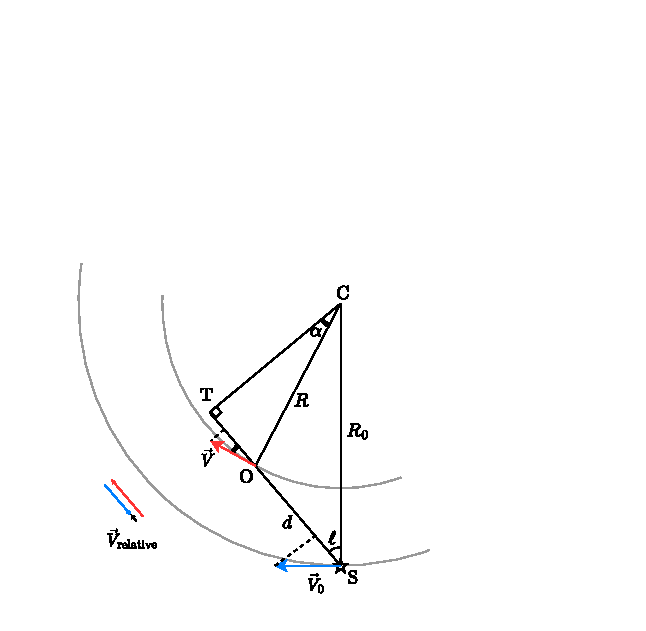
\includegraphics[width=0.5\textwidth]{figures/inner_circle_method.pdf}
    \caption{Schematic of the inner circle method}
    \label{fig:inner_circle_method}
\end{figure}
%
The velocity of the observed galactic object O given the relative velocity $V_r$ projected on the line of sight axis ST between the observer S and the object is given by
\begin{equation}
    V = \frac{R}{R_0} \left( \frac{V_r}{\sin(\ell)} + V_0 \right)
\end{equation}
\begin{proof}
    Using trigonometry, the distance TC can be written as
    \begin{equation}
       \textrm{TC} = R_0 \sin\ell = R \cos\alpha
       \label{eq:proof1}
    \end{equation}
    % and
    % \begin{equation}
    %     \textrm{TO} = R_0 \cos\ell - d = R \sin\alpha
    %    \label{eq:proof2}
    % \end{equation}
    The projected relative velocity is given by
    \begin{equation}
        V_r = V \cos\alpha - V_0 \sin\ell
       \label{eq:proof3}
    \end{equation}
    From \autoref{eq:proof1}, it is clear that $\cos\alpha = \frac{R_0}{R} \sin\ell$. Substituting in \autoref{eq:proof3}, we get
    \begin{equation}
        V_r = \left( \frac{R_0}{R} V - V_0 \right) \sin\ell
    \end{equation}
    By rearanging this equation, the final result can be found
    \begin{equation}
        V = \frac{R}{R_0} \left( \frac{V_r}{\sin(\ell)} + V_0 \right)
    \end{equation}
\end{proof}

\section{Estimating distance with the general equation}
\label{sec:distance_with_tangent_method}
Given an estimate for the radius $R$ of the orbit, the distance $d$ between the observer and the object can be estimated. Using the law of cosines, we can link the radius $R$ to the distance $d$:
\begin{equation}
    R^2 = R_0^2 + d^2 - 2 R_0 d \cos(\ell)
\end{equation}
This gives a second degree equation for $d$, with solutions
\begin{equation}
    d_\pm = \frac{2R_0 \cos(\ell) \pm \sqrt{4R_0^2 \cos^2(\ell) - 4(R_0^2 - R^2)}}{2} = R_0 \cos(\ell) \pm \sqrt{R^2 - R_0^2 \sin^2(\ell)}
\end{equation}
There are multiple cases: for $90^\circ < \ell < 270^\circ$, only the positive solution $d_+$ has physical significance, as the observed target cannot be behind the Sun. For $\ell < 90^\circ$, the two solutions are feasable and another method must be used to determine the correct solution. One way would be to make a measurement at a slightly different galactic latitude. If the peak yielding this distance estimate is still present, it means that the observed cloud was relatively close, and the $d_-$ solution can be retained. If the peak disapears, it means the distance must be large, and the $d_+$ solution can be retained.

\section{Oort constants method}
\label{sec:oort_method}

\begin{proof}
    Let $V_r$ and $V_t$ be the component along the line of sight and perpendicular to the line of sight of the relative velocity between the object and the observer $\vec V_\textrm{relative} = \vec V - \vec V_0$. From the Oort constants, the distance $d$ between the observer and the object is
    \begin{equation}
        d = \frac{V_r}{A \sin(2\ell)}
    \end{equation}
    Using the second Oort constant $B = \frac{V_r}{d} - A \cos(2\ell)$, the transverse component can be expressed as
    \begin{equation}
        V_t = d (B + A \cos(2\ell))
    \end{equation}
    To obtain the angular velocity of the object, the velocity of the observer, along and perpendicular to the line of sight, must simply be added to each component:
    \begin{align}
        V_{\parallel} &= V_r + V_0 \sin(\ell) \\
        V_{\perp} &= V_t - V_0 \cos(\ell)
    \end{align}
    The norm then gives the angular velocity:
    \begin{equation}
        \begin{aligned}
            V &= \sqrt{(V_r + V_0 \sin(\ell))^2 + (V_t - V_0 \cos(\ell))^2} \\
            &= \sqrt{(V_r + V_0 \sin(\ell))^2 + (d (B + A \cos(2\ell)) - V_0 \cos(\ell))^2}
        \end{aligned}
    \end{equation}
\end{proof}

\section{Example fit on measured spectrum}
\label{sec:fittings}

\begin{figure}[htbp]
    \centering
    \begin{subfigure}{0.49\textwidth}
        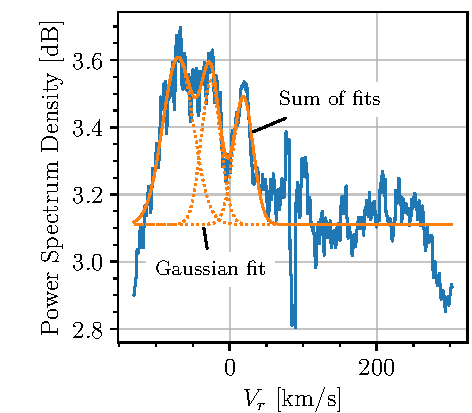
\includegraphics{figures/VEGA2_fit_l_127.pdf}
        \caption{}
        \label{fig:fit_VEGA}
    \end{subfigure}
    \begin{subfigure}{0.49\textwidth}
        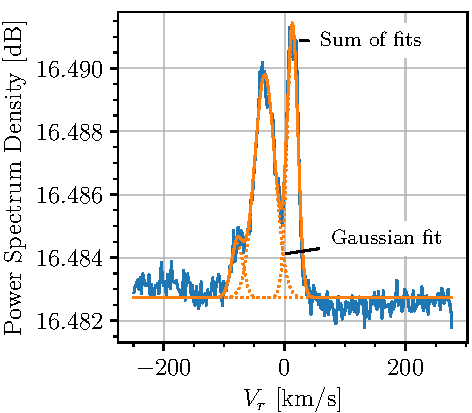
\includegraphics{figures/SALSA_fit_l_124.9.pdf}
        \caption{}
        \label{fig:fit_SALSA}
    \end{subfigure}
    \caption{Method used for finding the HI peaks. The mean of each fitted gaussian corresponds to the radial relative velocity of a hydrogen cloud. Showing measurement for (a) VEGA at $\ell = (127 \pm 1)^\circ$ and (b) SALSA at $\ell = (149.1 \pm 1.0)^\circ$}
    \label{fig:look_at_these_fits_please}
\end{figure}